\documentclass[xcolor=table,hideothersubsections]{beamer}
\usepackage[utf8]{inputenc}

%\documentclass[xcolor=table,hideothersubsections,aspectratio=1610]{beamer}
%should do exactly that. Other possible values are: 1610, 169, 149, 54, 43 and 32.
%By default, it is to 128mm by 96mm(4:3).

\usefonttheme{structurebold}

\useoutertheme[height=36pt,width=0cm]{sidebar}
\usetheme{Berkeley}

%\usetheme[width=1.65cm]{Berkeley}

\beamertemplatenavigationsymbolsempty

\uselanguage{French}
\languagepath{French}
\useinnertheme{rounded}

\usepackage{color, colortbl}
\usepackage{tcolorbox}
\usepackage{multirow}
\usepackage{textcomp}
\usepackage{siunitx}
\usepackage{tikz}
\usepackage[safe]{tipa}
\usepackage{array}
\usepackage{hhline}
\usepackage{pbox}
\usepackage{etoolbox}
\usepackage{algorithm,algorithmic}

\usepackage{environ}

\tikzset{rndblock/.style={rounded corners,rectangle,draw,outer sep=0pt}}
\newcommand{\tframed}[2][]{\tikz[baseline=0.1pt]\vspace{0.1cm}\node[rndblock,minimum height=1.5em,#1] (m) {#2} ;}
\newcommand{\hilight}[1]{\textbf{\tframed[blue,fill=blue!10]{#1}}}
\newcommand{\whilight}[1]{\textbf{\tframed[purple,fill=purple!10]{#1}}}

% tkiz ball item
\newcommand*\circled[1]{\tikz[baseline=(char.base)]{\node[circle,ball color=darkcerulean, shade,
 color=white,inner sep=2.2pt] (char) {\tiny #1};}}

% tkiz rounded item
\newcommand*\rounded[1]{\tikz[baseline=(char.base)]{\node[draw=none,ball color=darkcerulean, shade,
 color=white, rounded corners=3.5pt, inner sep=2.5pt] (char) {\scriptsize #1};}}

%==============================================================================================================

\newcommand{\sP}{\hspace{1pt}}
\newcommand{\mP}{\hspace{3pt}}
\newcommand{\bP}{\hspace{6pt}}
\newcommand{\BP}{\hspace{12pt}}

\newcommand\fontJ{\fontfamily{ptm}\fontsize{6.1}{7.2}\selectfont}

\newcolumntype{L}[1]{>{\raggedleft\let\newline\\\arraybackslash\hspace{0pt}}m{#1}}
\newcolumntype{g}{>{\columncolor{tgray}}S[tabformat=2.2]}

%==============================================================================================================
\definecolor{darkcerulean}{rgb}{0.03, 0.27, 0.49}
\definecolor{bluepigment}{rgb}{0.2, 0.2, 0.6}
\definecolor{cobalt}{rgb}{0.0, 0.28, 0.67}
\definecolor{clearblue}{RGB}{135,206,250}
\definecolor{blendedblue}{rgb}{0.137,0.466,0.741}
\definecolor{defaultB}{rgb}{0.03, 0.27, 0.49}
\definecolor{darksalmon}{RGB}{233,150,122}
\definecolor{blendedgray}{rgb}{0.838,0.833,0.833}
\definecolor{blendedpurple}{RGB}{75,20,130}
\definecolor{tgray}{rgb}{0.211, 0.211,0.244}
\definecolor{darkgray}{rgb}{0.450,0.450,0.450}
\definecolor{maroon}{rgb}{0.665, 0.142, 0.142}
\definecolor{ngreen}{rgb}{0.000,0.500,0.000}


\newcommand{\rul}[1]{\textcolor{cobalt}{\underline{\textcolor{cobalt}{#1}}}}
\newcommand{\wul}[1]{\textcolor{white}{\underline{\textcolor{black}{#1}}}}

%==============================================================================================================
\newlength\leftsidebar
\newlength\rightsidebar
\makeatletter
\setlength\leftsidebar{\beamer@leftsidebar}
\setlength\rightsidebar{\beamer@rightsidebar}
\makeatother


%show current section and subsection
\makeatletter
\patchcmd{\insertverticalnavigation}%
{\ifx\beamer@nav@css\beamer@hidetext{\usebeamertemplate{section in sidebar}}\else{\usebeamertemplate{section in sidebar shaded}}\fi}%
{{\usebeamertemplate{section in sidebar}}}{}{}
\makeatother


% itemize
\setbeamercolor{item projected}{bg=darkcerulean}

\setbeamertemplate{itemize item}{\raise3.4pt\hbox{\donotcoloroutermaths\circled{}}}
\setbeamertemplate{itemize subitem}{\scriptsize\raise0.5pt\hbox{\donotcoloroutermaths\color{darkcerulean}$\ast$}}
\setbeamertemplate{itemize subsubitem}{\scriptsize\raise0.5pt\hbox{\donotcoloroutermaths\color{darkcerulean}$\triangleright$}}
\setbeamertemplate{itemize/enumerate subbody begin}{\footnotesize}
\setbeamertemplate{itemize/enumerate subsubbody begin}{\scriptsize}

\setlength{\leftmargini}{10pt}
\setlength{\leftmarginii}{10pt}

%==============================================================================================================
\setbeamerfont{footline}{series=\bfseries}
\setbeamercolor{footline}{fg=darkcerulean}

\setbeamercolor{section in toc}{fg=darkcerulean}
\setbeamercolor{section number projected}{fg=white,bg=darkcerulean}

\setbeamercolor{section in toc shaded}{fg=darkcerulean!50}
\setbeamercolor{section in sidebar shaded}{fg=darkcerulean!80}
\setbeamercolor{subsection in sidebar shaded}{fg=darkcerulean!80}

\setbeamercolor{sidebar}{fg=white,bg=darkcerulean}
\setbeamercolor{author in sidebar}{fg=clearblue}
\setbeamercolor{title in sidebar}{fg=clearblue}

\setbeamercolor{palette primary}{fg=white,bg=darkcerulean}
\setbeamercolor{palette secondary}{fg=white,bg=darkcerulean!108}
\setbeamercolor{palette structure}{fg=white,bg=darkcerulean}

\setbeamercolor{itemize item}{fg=darkcerulean,bg=darkcerulean}


%==============================================================================================================
\addtobeamertemplate{navigation symbols}{}{%
    \usebeamerfont{footline}%
    \usebeamercolor[fg]{footline}%
    \hspace{1em}%
    \insertframenumber/\inserttotalframenumber
}

\setbeamercolor{lowcol}{fg=black,bg=darkcerulean!30}

\newenvironment{titleblock}{
  \setbeamercolor{block title}{fg=white,bg=darkcerulean}
  \setbeamercolor{block body}{fg=white,bg=darkcerulean}
  \begin{beamerboxesrounded}[width=1.05\textwidth,shadow=true]
}{\end{beamerboxesrounded}}

\newenvironment<>{varblock}[2][\textwidth]{%
\vspace*{-20pt}
	  \setlength{\textwidth}{#1}
	  \begin{actionenv}#3%
	    \def\insertblocktitle{#2}%
	    \par%
	    \usebeamertemplate{block begin}}
	  {\par%
	    \usebeamertemplate{block end}%
	  \end{actionenv}
\vspace*{-20pt}
}

\newenvironment{variableblock}[3]{%
  \setbeamercolor{block body}{#2}
  \setbeamercolor{block title}{#3}
  \begin{block}{#1}
}{\end{block}}



%%%%%%%%%%%%%%%%%%%%%%%%%%%%%%%%%%%%%%%%%%%%%%%%%%%%%%%%%%%%%%%%%%%%%%%%%%%%%

\NewEnviron{specialannexe}[1][]{%
\begingroup
	\setbeamertemplate{footline}[frame number]{}
	\setbeamertemplate{navigation symbols}{}
	\setbeamertemplate{footline}{}

	\setbeamercolor{palette secondary}{fg=white,bg=darkcerulean}

	\makeatletter
	\setbeamertemplate{sidebar canvas left}{}
	\setbeamertemplate{sidebar left}{%
	  \vspace*{\fill}
	  \vspace*{\fill}
	}
	\makeatother

	\begin{frame}[noframenumbering,t]{\hskip-11ex Annexe}
	\makebox[\textwidth][c]{
	\begin{minipage}{\dimexpr\textwidth+0.25\textwidth\relax}
	\BODY
	\end{minipage}}
	\end{frame}
\endgroup
}

%%%%%%%%%%%%%%%%%%%%%%%%%%%%%%%%%%%%%%%%%%%%%%%%%%%%%%%%%%%%%%%%%%%%%%%%%%%%%

\newenvironment{specialframe}{%
    \begingroup
    \setbeamertemplate{navigation symbols}{}
    \begin{frame}[noframenumbering,plain]
}{\end{frame}
    \addtobeamertemplate{navigation symbols}{}{%
	\usebeamerfont{footline}%
	\usebeamercolor[fg]{footline}%
	\hspace{1em}%
	\insertframenumber/\inserttotalframenumber}
\endgroup}

\makeatletter
\long\def\beamer@@frametitle[#1]#2{%
  \beamer@ifempty{#2}{}{%
    \gdef\insertframetitle{\centering{#2\ifnum\beamer@autobreakcount>0\relax{}\space\usebeamertemplate*{frametitle continuation}\fi}}%
  \gdef\beamer@frametitle{#2}%
  \gdef\beamer@shortframetitle{#1}%
}%
}
\makeatother


%==============================================================================================================
% TOC
%==============================================================================================================

\AtBeginSection[]
{
	\hoffset=-.5\leftsidebar
	\begin{specialframe}
		\vskip-6ex
		\begin{variableblock}{}{bg=darkcerulean,fg=white}{}
		  \vskip1pt\hskip5pt\Large{\textbf{\color{white} Sommaire}}
		\end{variableblock}

		\vskip3ex

		\begin{minipage}{\textwidth}
			\vskip1\baselineskip
			\fontsize{10}{25}\selectfont
			\tableofcontents[currentsection, sectionstyle=show/shaded, hideothersubsections, subsectionstyle=hide/hide/hide]
			\vskip0pt plus 1filll

		\end{minipage}

	\end{specialframe}
	\hoffset=0ex
}


%==============================================================================================================
% First slide
%==============================================================================================================
\title[RAPSODIE]{\vskip0.4ex Application for the Post Doc Position \\in Speech Recognition \\\vskip0.3ex(Malorca project)}
\author[Luiza Orosanu]{\textbf{\large Luiza Orosanu}\vskip-1cm}
\date{\footnotesize 5th February 2016}

\newcommand{\firstslide}
{
   \hoffset=-.5\leftsidebar
   \begin{specialframe}
	\begin{center}

	\vskip1ex
	\begin{titleblock}{}
	\centering\usebeamerfont{title}\inserttitle\par
	\end{titleblock}

	\vskip5ex
	\usebeamerfont{author}\insertauthor\par

	\vskip8ex
	INRIA-Loria, Nancy, France

	\vskip3ex
	\usebeamerfont{date}\insertdate\par

	\end{center}

	\vskip-2ex
	\begin{table}[h]
	\hspace*{0.5ex}\begin{tabular}{ccccc}
	
\includegraphics{Image/logos/logo-LORIA.pdf} & 
\includegraphics[scale=0.2]{Image/logos/logo-INRIA.pdf} & 
\includegraphics[scale=0.6]{Image/logos/logo-UL.pdf}  & & 
\includegraphics[scale=0.09]{Image/logos/logo-CNRS.pdf}
	\end{tabular}
	\end{table}

	\vskip-3ex
   \end{specialframe}
   \hoffset=0ex
}


%==============================================================================================================
% document
%==============================================================================================================

\begin{document}
\firstslide

%==============================================================================================================
\begin{frame}{Short introduction}

\only<1>
{
\footnotesize
\hspace*{-6.1ex}
\renewcommand{\arraystretch}{1.2}\begin{tabular}{|p{2.3cm}|p{2.5cm}|p{2.9cm}|p{2.9cm}|}
\hline
\textbf{2006 \hskip4.92ex -2010} 	& \multicolumn{1}{r|}{\textbf{-2011}}	&  \multicolumn{1}{r|}{\textbf{-2012}}	& \multicolumn{1}{r|}{\textbf{-2015}}			\\ \hline
\multicolumn{1}{|l|}{\textbf{\color{purple}BSc} in} 	&     				&  					& 		  				\\
\multicolumn{1}{|l|}{computer science} 	&  					&  					& 		  					\\
 					& \multicolumn{1}{l|}{\textbf{\color{purple}MSc} in}		&			&		  				\\
 					& \multicolumn{1}{l|}{computer science}	&					&		  					\\
 					& 					& \multicolumn{1}{l|}{\textbf{\color{purple}Engineer:}}	&  					\\
 					& 					& \multicolumn{1}{l|}{ALLEGRO project}	&  							\\
 					& 					& 					&  \multicolumn{1}{l|}{\textbf{\color{purple}PhD student:}} \\
 					& 					& 					&  \multicolumn{1}{l|}{RAPSODIE project}		\\
 					& 					& 					&  							\\ \hline
{\scriptsize head tracking}		& {\scriptsize speech recognition} 	& {\scriptsize incorrect entries}	& {\scriptsize \wul{hybrid language models}}		\\
{\scriptsize Wii remote}		& {\scriptsize remote sound}		& {\scriptsize non-native speech}	& {\scriptsize \wul{add new words}}			\\
{\scriptsize infrared sensors}		& {\scriptsize adaptation}		& {\scriptsize speech-text alignments}	& {\scriptsize question detection}			\\ \hline
{\scriptsize \color{darkcerulean} \vskip-2.5ex Romania}	& \multicolumn{3}{c|}{\scriptsize \color{darkcerulean} France}								\\ \hline
\end{tabular}
}

\only<2->
{
\footnotesize
\hspace*{-6.1ex}
\renewcommand{\arraystretch}{1.2}\begin{tabular}{|p{2.3cm}|p{2.5cm}|p{2.9cm}|p{2.9cm}|}
\hline
\textbf{2006 \hskip4.92ex -2010} 	& \multicolumn{1}{r|}{\textbf{-2011}}	&  \multicolumn{1}{r|}{\textbf{-2012}}	& \multicolumn{1}{r|}{\textbf{-2015}}				 \\ \hline
\multicolumn{1}{|l|}{\textbf{\color{purple}BSc} in} 	&     			&  					& 		  						 \\
\multicolumn{1}{|l|}{computer science} 	&  					&  					& 		  						 \\
 					& \multicolumn{1}{l|}{\textbf{\color{purple}MSc} in}		&		&		  					 	 \\
 					& \multicolumn{1}{l|}{computer science}	&					&		  						 \\
 					& 					& \multicolumn{1}{l|}{\textbf{\color{purple}Engineer:}}	&  						 \\
 					& 					& \multicolumn{1}{l|}{ALLEGRO project}	&  								 \\
 					& 					& 					&  \multicolumn{1}{l|}{\textbf{\color{purple}PhD student:}} 	 \\
 					& 					& 					&  \multicolumn{1}{l|}{RAPSODIE project}			 \\
 					& 					& 					&  								\\ \hline
{\scriptsize head tracking}	& {\scriptsize speech recognition} 	& {\scriptsize incorrect entries}		& {\scriptsize \rul{hybrid language models}} 			\\
{\scriptsize Wii remote}		& {\scriptsize remote sound}		& {\scriptsize non-native speech}	& {\scriptsize \rul{add new words}} 	 			\\
{\scriptsize infrared sensors}		& {\scriptsize adaptation}		& {\scriptsize speech-text alignments}	& {\scriptsize question detection}				 \\ \hline
{\scriptsize \color{darkcerulean} \vskip-2.5ex Romania}	& \multicolumn{3}{c|}{\scriptsize \color{darkcerulean} France}									 \\ \hline
\end{tabular}
}

\end{frame}

%==============================================================================================================
\section{Hybrid language models}
\begin{frame}[t]{Hybrid language models}

\begin{itemize}
\vskip2.5ex
\item \textbf{\color{purple}Context}

	\begin{itemize}
	\vskip3ex
	\item \textbf{\color{blendedblue}OOV words} (regardless the size of vocabulary)

		\vskip2ex
		\hskip4ex\begin{beamerboxesrounded}[width=0.88\textwidth,shadow=true]{}
		\footnotesize
		\begin{center}
			\begin{tabular}{lcccccc}
			Reference: 	& dans & un & \multicolumn{2}{c}{village} 	& du & nord  \\
			Hypothesis: 	& dans & {\color{red}++parole++} & {\color{red}l'} & {\color{red}âge} & du & nord
			\end{tabular}
		\end{center}
		\end{beamerboxesrounded}

	\vskip2.5ex
	\item maximize the \textbf{\color{blendedblue}understanding of the resulting transcription}\\\vskip0.4ex for the deaf community

	\end{itemize}

\vskip4ex
\item \textbf{\color{purple}Hybrid language models}
	\begin{itemize}
	\vskip3ex
	\item combining words with word-fragments
	\end{itemize}

\end{itemize}

\end{frame}

%==============================================================================================================
\subsection{Approach}
\begin{frame}[t]{Approach}

\begin{itemize}
\vskip3ex
\item<1-> Choice of a \textbf{\color{purple}hybrid language model of words \& syllables}
	\begin{itemize}
	\vskip1ex
	\item ensure the \textbf{\color{blendedblue}proper recognition of the most frequent words}

	\vskip1ex
	\item provide a sequence of syllables for out-of-vocabulary words

     	\vskip2ex
	\hskip1ex\begin{beamerboxesrounded}[width=0.88\textwidth,shadow=false]{}
	\begin{center}
		{\color{purple}{\fontencoding{U}\fontfamily{futs}\selectfont\char 66\relax}}
	     		syllables trained on \textbf{\color{blendedblue}real pronunciations} \\
		\vskip0.7ex (1 syllable $=$ 1 single sequence of phonemes $=$ 1 pronunciation)
	\end{center}
	\end{beamerboxesrounded}

	\end{itemize}

\vskip3ex
\item<2-> Motivations
	\begin{itemize}
	\vskip1ex
	\item \textbf{\color{purple} syllables} {\color{darkcerulean}$\longleftarrow$} study on optimising the phonetic decoding

	\vskip1ex
	\item \textbf{\color{purple} words} \hskip2.7ex {\color{darkcerulean}$\longleftarrow$} interviews conducted with deaf people
	\end{itemize}
\end{itemize}

\only<3->
{
	\vskip1ex
	\hskip6ex\begin{beamerboxesrounded}[width=0.8\textwidth,shadow=true]{Example of a hybrid transcription}
	\footnotesize
	\begin{center}
		\begin{tabular}{ll}
		Decoding:  & une femme a été \ \_\textipa{b}\_\textipa{l}\_\textipa{e} \ \_\textipa{s}\_\textipa{e}  \\
		Display:   & une femme a été \ \textipa{b} \textipa{l} \textipa{é} \textipa{s} \textipa{é}
		\end{tabular}
	\end{center}
	\end{beamerboxesrounded}
}


\end{frame}

%==============================================================================================================
\begin{frame}[t]{Syllabification}

\begin{itemize}
\vskip1ex
\item<1-> Training corpus for hybrid language models
	\begin{itemize}
	\vskip1.5ex
	\item {\footnotesize keep only the \textbf{\color{purple}most frequent words} {\color{gray}\scriptsize ($\#occ \ge N$)}}
	\vskip1.5ex
	\item {\footnotesize \textbf{\color{purple}syllabify} the other words (less frequent)}
	\end{itemize}

\vskip2.5ex
\item<2-> Syllabification
	\begin{itemize}
	\vskip1.5ex
	\item forced alignement \textbf{\color{purple}words $\rightarrow$ phonemes}

	\vskip1.5ex
	\item syllabification rules \textbf{\color{purple}phonemes $\rightarrow$ syllables} \scriptsize{\color{blendedblue}[Bigi et al. 2010]}

	\only<3->
	{
		\begin{itemize}
		\vskip1ex
		\item {\scriptsize a syllable contains a single vowel {\color{darkcerulean}(V)}}

		\vskip1ex
		\item {\scriptsize a pause designates a syllable's boundary}
		\end{itemize}

		\vskip3ex
		{\scriptsize
		\hspace*{0.5ex}\begin{tabular}{|c|c|c|lr|}
		\hline
		\textbf{Rule}    & \textbf{Sequence of}	  	& \textbf{Split}  	& \multicolumn{2}{c|}{\textbf{Resulting}}     	\\
		\textbf{type}    & \textbf{phonetic classes} 	& \textbf{position} 	& \multicolumn{2}{c|}{\textbf{syllables}}  	\\ \hline
		GEN		 & {\color{darkcerulean}VV} 				& 0 	& {\color{darkcerulean}V}   & {\color{darkcerulean}V}	\\
		GEN		 & {\color{darkcerulean}V}x{\color{darkcerulean}V} 	& 0 	& {\color{darkcerulean}V}   & x{\color{darkcerulean}V}	\\
		GEN		 & {\color{darkcerulean}V}xx{\color{darkcerulean}V} 	& 1 	& {\color{darkcerulean}V}x  & x{\color{darkcerulean}V}	\\\hline
		EXC 		 & {\color{darkcerulean}V}OL{\color{darkcerulean}V}	& 0 	& {\color{darkcerulean}V}   & OL{\color{darkcerulean}V}	\\\hline
		\end{tabular}
		}
	}

	% diplomatie = d i p l oh m a s i = O V O L V O V O V = OV | OLV | OV | OV = d i | p l oh | m a | s i

	\end{itemize}
\end{itemize}

\end{frame}

%==============================================================================================================
\begin{frame}[t]{Syllabification}

\begin{center}
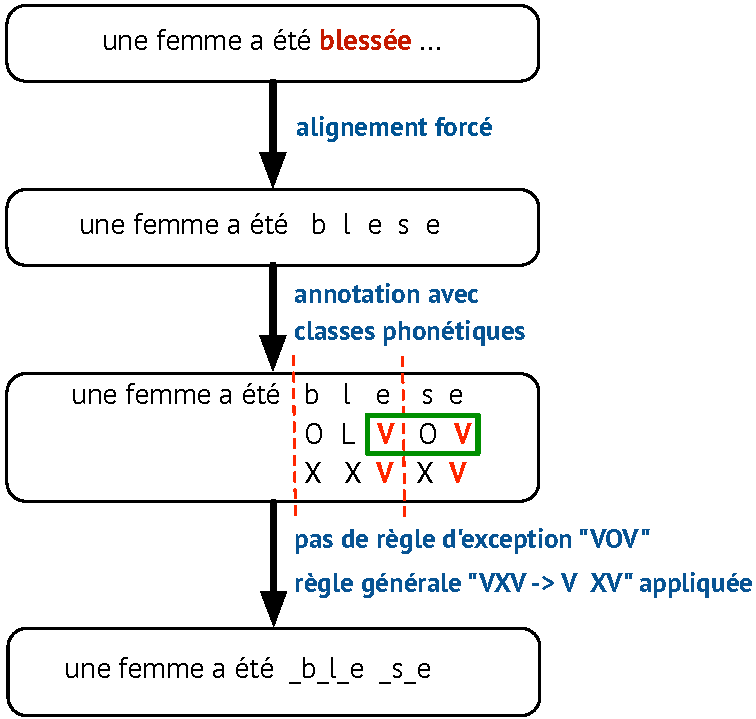
\includegraphics[scale=0.5]{Image/picture/syllabation-WS.pdf}
\end{center}

\end{frame}


%==============================================================================================================
\subsection{Experiments}
\begin{frame}[t]{Evaluation of hybrid language models}

\vskip2ex
\hskip6ex\begin{beamerboxesrounded}[width=0.8\textwidth,shadow=false]{}
	\footnotesize
	\begin{center}
		\begin{tabular}{ll}
		Word-based model: 	& une femme a été blessée \\
		Hybrid model: 		& une femme a été \ \_b\_l\_e \ \_s\_e \\
		\end{tabular}
	\end{center}
	\end{beamerboxesrounded}


\begin{itemize}
\vskip4ex
\item \textbf{\color{purple}Performance of hybrid models}
	\begin{itemize}
	\vskip1.5ex
	\item phoneme error rate
	\vskip1.5ex
	\item percentage of words in the automatic transcription
	\vskip1.5ex
	\item percentage of correctly recognized words and syllables
	\vskip1.5ex
	\item percentage of out-of-vocabulary words recognized as syllables
	\end{itemize}

\vskip4ex
\item Apply a filter on the \textbf{\color{purple}confidence measure of words}
	\begin{itemize}
	\vskip1.5ex
	\item[$\rightarrow$] phonetize words with low confidence measures
	\end{itemize}

\end{itemize}


\end{frame}

%==============================================================================================================
\subsection{Conclusions}
\begin{frame}[t]{Conclusions}

\begin{itemize}

\vskip3ex
\item our hybrid modeling solution takes into acount \\ \textbf{\color{purple}real pronunciations}

\vskip3ex
\item the speech recognition outputs contain mainly words

\vskip3ex
\item over 70\% of words are correctly recognized

\vskip3ex
\item the confidence measures can effectively select the \\correctly recognized words

\vskip3ex
\item an increased amount of syllables in the training corpus
	\begin{itemize}
	\vskip0.3ex \item improves the percentage of correctly recognized syllables
	\vskip0.3ex \item improves the percentage of OOV words decoded as syllables
	\end{itemize}
\end{itemize}

\end{frame}


%==============================================================================================================
\section{Adding new words to a language model}
\begin{frame}[t]{Adding new words to a language model}

\begin{itemize}
\vskip7ex
\item \textbf{\color{purple}Context}
	\begin{itemize}
	\vskip2ex
	\item OOV words that are frequently pronounced
		\begin{itemize}
		\vskip1ex
		\item ex: words specific to a certain area
		\end{itemize}
	\end{itemize}

\vskip5ex
\item \textbf{\color{purple}Adding new words to an ASR system involves}
	\begin{itemize}
	\vskip2ex
	\item generating the pronunciation variants
	\vskip2ex
	\item modifying the language model
	\end{itemize}
\end{itemize}

\end{frame}

%==============================================================================================================
\subsection{Approach}
\begin{frame}[t]{Approach}

\begin{itemize}
\vskip4ex
\item without retraining or adapting the model \\(which requires a lot of new data relative to the new words)

\vskip4ex
\item approach based on the similarity between words

	\vskip2ex
	\begin{center}
	\hspace{-0.2cm}\begin{beamerboxesrounded}[width=0.79\textwidth,shadow=false]{}
		{\footnotesize
		\begin{tabular}{rcl}
			on ignorait encore lundi & \hskip-1.7ex \textbf{\color{purple}soir}  & \hskip-1.7ex les conditions de sa survie \\
			on ignorait encore lundi & \hskip-1.7ex \textbf{\color{ngreen}matin} & \hskip-1.7ex les conditions de sa survie \\
		\end{tabular}
		}
	\end{beamerboxesrounded}
	\end{center}

	\only<2->
	{
		\begin{itemize}
		\vskip3ex
		\item[$\rightarrow$] use \textbf{\color{blendedblue}a few examples of sentences} for each new word
		\vskip2ex
		\item[$\rightarrow$] find similar known words ({\color{blendedblue}having similar neighbor distributions})
		\vskip2ex
		\item[$\rightarrow$] \textbf{\color{blendedblue}transpose the LM probabilities} of known words onto the new words
		\end{itemize}
	}

\end{itemize}


\end{frame}




%==============================================================================================================
\begin{frame}[t]{Neighbors of new words}

\begin{itemize}
\vskip-1ex
\item[\textbf{\color{blendedblue}1.}] Use a few \textbf{\color{blendedblue}examples of sentences} with the new word

	{\footnotesize
	\vskip1ex \hskip-0.5ex $\rightarrow$ compute the neighbor distributions of the new word \textbf{\color{purple}nW}
	\begin{center}$P_k(w|\textbf{\color{purple}nW}) \text{ for } k \in \{..., -2, -1, +1, +2, ...\}$\end{center}
	}
\end{itemize}

\vskip1ex

\only<2->
{
\footnotesize
\vskip-1ex{\color{darkcerulean}\rule{\textwidth}{0.9pt}}

\begin{itemize}

\vskip-1ex
\item example of a new word: \textbf{\color{purple}soir}

\vspace*{1ex}
\item examples of sentences

	\vspace*{-2.5ex}
	\begin{center}
	{\scriptsize
	\hspace*{-4ex}\begin{tabular}{rcccccl}
	 	   	   & {\color{blendedblue}$-2$} & {\color{blendedblue}$-1$} & & {\color{blendedblue}$+1$}  & {\color{blendedblue}$+2$}  & 	\\\cline{2-6}
	on ignorait 	   & \underline{encore} & \underline{lundi} 	& \textbf{\color{purple}soir} & \underline{les} & \underline{conditions} & de sa survie \\
	devine qui vient   & \underline{dîner}  & \underline{ce}    	& \textbf{\color{purple}soir} & & &  \\
	pas de consigne de & \underline{vote} 	& \underline{au} 	& \textbf{\color{purple}soir} & \underline{du}  & \underline{premier} 	 & tour \\
	\end{tabular}
	}
	\end{center}

\vspace*{1ex}
\item preceding and succeeding neighbors \hskip0.5ex
	{\scriptsize
	\begin{tabular}{l|l}
	$k= -2$  	& encore, dîner, vote,  ... 	\\
	$k= -1$  	& lundi, ce, au, ... 		\\
	$k= +1$  	& les, du, ...    		\\
	$k= +2$  	& conditions, premier, ... 	\\
	\end{tabular}
	}

\end{itemize}

}

\end{frame}

%==============================================================================================================
\begin{frame}[t]{Neighbors of known words}

\begin{itemize}
\vskip-1ex
\item[\textbf{\color{blendedblue}2.}] Search for similar words in a \textbf{\color{blendedblue}reference corpus}

	{\footnotesize
	\vskip1ex\hskip-0.5ex $\rightarrow$ compute the neighbor distributions of each known word \textbf{\color{ngreen}kW}
	\begin{center}$P_k(w'|\textbf{\color{ngreen}kW}) \text{ for } k \in \{..., -2, -1, +1, +2, ...\}$\end{center}
	}
\end{itemize}

\vskip0.3ex

\only<2->
{
\footnotesize
\vskip-1ex{\color{darkcerulean}\rule{\textwidth}{0.95pt}}

\begin{itemize}
\item use directly the n-gram counts file
	\begin{itemize}
	\vspace*{0.1ex}
	\item {\scriptsize 3-gram $\Rightarrow$ maximum 4 neighbors $k \in \{-2,-1,+1,+2\}$}
	\end{itemize}

\vspace*{2ex}
\item examples of 3-gram entries with the known word `\textbf{\color{ngreen}matin}'

	\vskip1ex
	\begin{columns}
	\begin{column}{0.5\textwidth}
		{\scriptsize\fontfamily{qcr}\selectfont
		\renewcommand{\arraystretch}{1.01}
		\begin{tabular}{cccr}
		\hskip3ex "\textbf{\color{ngreen}matin} 	& a 				& été 				& \textit{10}" 	\\
		\hskip3ex "beau 				& \textbf{\color{ngreen}matin} 	& de 				& \textit{9}" 	\\
		\hskip3ex "jusqu' 				& au 				& \textbf{\color{ngreen}matin} 	& \textit{28}" 	\\
		\end{tabular}
		}
	\end{column}
	\begin{column}{0.5\textwidth}
		\vskip-1ex
		{\tiny
		\renewcommand{\arraystretch}{1.5}
		\begin{tabular}{ll}
		$\rightarrow$ voisin $k=+1$ `a'; 	& \hskip-3ex voisin $k=+2$ `été' 	\\
		$\rightarrow$ voisin $k=-1$ `beau'; 	& \hskip-3ex voisin $k=+1$ `de' 	\\
		$\rightarrow$ voisin $k=-2$ `jusqu'; 	& \hskip-3ex voisin $k=-1$ `au'
		\end{tabular}
		}
	\end{column}
	\end{columns}


\vspace*{2ex}
\item preceding and succeeding neighbors \hskip1ex
	{\scriptsize
	\begin{tabular}{l|l}
	$k= -2$  	& jusqu', ... 		\\
	$k= -1$  	& beau, au, ... 	\\
	$k= +1$  	& de, a, ...    	\\
	$k= +2$  	& été, ... 		\\
	\end{tabular}
	}
\end{itemize}

}

\end{frame}


%==============================================================================================================
\begin{frame}[t]{Word similarity}


\begin{itemize}
\vskip1ex
\item[\textbf{\color{blendedblue}3.}] Compute the \textbf{\color{blendedblue}KL divergence} between the neighbor distributions \\
	{\footnotesize \vskip1ex$\rightarrow$  between each known word (\textbf{\color{ngreen}kW}) and the new word (\textbf{\color{purple}nW})}

	\vskip1.5ex
	\begin{center}
	\hspace{-0.2cm}\begin{beamerboxesrounded}[width=0.93\textwidth,shadow=false]{}
		{\footnotesize {\color{purple}Divergence computed on each $k$ position:} }

		\vskip1ex
		{\scriptsize
		\renewcommand{\arraystretch}{1.5}
		\hskip4ex \begin{tabular}{rp{0.01cm}l}
		\hskip-0.3ex $D_{KL} \left( \ P_{k}(\bullet|\textbf{\color{ngreen}kW}) \ || \ {P_{k}(\bullet|\textbf{\color{purple}nW})}\ \right)$
		& \hskip-2ex =
		& \hskip-2ex $\sum\limits_{w \in V(\textbf{\color{purple}nW})}^{ } \ P_{k}(w|\textbf{\color{ngreen}kW}) \ log \left( \frac{P_{k}(w|\textbf{\color{ngreen}kW})}{P_{k}(w|\textbf{\color{purple}nW})} \right)$ \\
		\end{tabular}
		}

		\vskip2.1ex
		{\footnotesize {\color{purple}Global divergence: } }

		\vspace*{-4.0ex}
		\begin{center}
		{\scriptsize $D(\textbf{\color{ngreen}kW},\textbf{\color{purple}nW})\ =\ \sum\limits_{k} D_{k}(\textbf{\color{ngreen}kW},\textbf{\color{purple}nW})$}
		\end{center}
	\end{beamerboxesrounded}
	\end{center}
\end{itemize}

\only<2->
{
	\begin{itemize}
	\vskip2ex
	\item[\textbf{\color{blendedblue}4.}] Select the \textbf{\color{blendedblue} mots similar words} to the new word
		{\footnotesize \vskip1ex \hskip3ex $\rightarrow$ those having minimal divergences}
	\end{itemize}
}

\vspace*{-2ex}
\only<3->
{
	\begin{center}
	\hspace{-0.2cm}\begin{beamerboxesrounded}[width=0.9\textwidth,shadow=false]{}
		{\scriptsize {\color{purple}Examples of similar words:} }

		\vskip0.9ex
		{\scriptsize
		\begin{tabular}{p{1.3cm}p{0.5cm}p{7cm}}
		& soir		& $\rightarrow$ \ matin, midi, dimanche, samedi, vendredi	\\
		& soirs		& $\rightarrow$ \ temps, joueurs, matchs, pays, matches	 	\\
		\end{tabular}
		}
	\end{beamerboxesrounded}
	\end{center}
}

\end{frame}


%==============================================================================================================
\begin{frame}[t]{Adding new n-grams}

\begin{itemize}

\vspace*{0.1ex}
\item[\textbf{\color{blendedblue}5.}] \textbf{\color{blendedblue}Transpose the n-gram probabilities} of similar words \\ \hskip2ex onto the new word

	\begin{itemize}
	\vskip1.5ex
	\item[$\rightarrow$] seek the n-grams that contain similar words

	\vskip1ex
	\item[$\rightarrow$] replace the 'similar words' with the 'new word'

	\vskip1ex
	\item[$\rightarrow$] add the new n-grams into the new language model
	\end{itemize}
\end{itemize}

\vskip0.1cm

\only<2->
{
\footnotesize
\vskip-1ex{\color{darkcerulean}\rule{\textwidth}{0.9pt}}


\begin{itemize}
\smallskip
\item new word "\textbf{\color{purple}soir}" similar to known word "\textbf{\color{ngreen}matin}"

\vskip2ex
\item \underline{known n-grams}  (in the language model) \\
	{\scriptsize
	\vskip1ex\hskip5ex {\scriptsize\fontfamily{qcr}\selectfont"-1.48214 possible ce \textbf{\color{ngreen}matin}"} \\
	\vskip1ex\hskip5ex {\scriptsize\fontfamily{qcr}\selectfont"-1.404164 \textbf{\color{ngreen}matin} ajoute que"}
	}

\vskip2ex
\item \underline{new n-grams} (to add into the new language model) \\
	{\scriptsize
	\vskip1ex\hskip5ex {\scriptsize\fontfamily{qcr}\selectfont"-1.48214 possible ce \textbf{\color{purple}soir}"} \\
	\vskip1ex\hskip5ex {\scriptsize\fontfamily{qcr}\selectfont"-1.404164 \textbf{\color{purple}soir} ajoute que"}
	}

\end{itemize}

}

\end{frame}





%==============================================================================================================
\subsection{Experiments}
\begin{frame}[t]{Setup for experiments}

\begin{itemize}
\vskip3ex
\item \textbf{\color{purple}44 new words} selected

\vskip4ex
\item Search for similar words
	\begin{itemize}
	\vskip2ex
	\item {\scriptsize sentences based on "\textbf{\color{orange}word}$|$POS" units}

		\vskip1ex
		\begin{columns}
		\begin{column}{0.1\textwidth}
		\end{column}
		\begin{column}{1.08\textwidth}
		\hspace*{6ex}
		\begin{beamerboxesrounded}[width=0.8\textwidth,shadow=false]{}
			{\scriptsize \  \textbf{\color{orange}qui}$|$PRO:REL \hskip1ex \textbf{\color{orange}vient}$|$VER:pres \hskip1ex \textbf{\color{orange}dîner}$|$VER:infi
			\hskip1ex \textbf{\color{orange}ce}$|$PRO:DEM \hskip1ex  \textbf{\color{orange}soir}$|$NOM }
		\end{beamerboxesrounded}
		\end{column}
		\end{columns}

	\vskip2ex
	\item {\scriptsize 4 neighbors for each word: $k \in \{-2, -1, +1, +2\}$}
	\end{itemize}

\vskip4ex
\item Evaluate the impact of
	\begin{itemize}
	\vskip1ex
	\item number of examples of sentences for each new word {\scriptsize (5, 10, 20 or 50) }
	\vskip0.5ex
	\item nomber of similar words for each new word {\scriptsize (5, 10, 20 or 50) }
	\end{itemize}
\end{itemize}

\end{frame}



%==============================================================================================================
\begin{frame}[t]{Setup for experiments}

\begin{itemize}

\vskip2ex
\item \textbf{\color{purple}BASELINE} language model
	\begin{itemize}
	\vskip0.5ex
	\item {\scriptsize large vocabulary language model trained by interpolation}
	\vskip0.1ex
	\item {\scriptsize the 44 new words are absent in this model}
	\end{itemize}


\vskip2ex
\item \textbf{\color{purple}ORACLE} language model
	\begin{itemize}
	\vskip0.5ex
	\item {\scriptsize large vocabulary language model trained by interpolation}
	\vskip0.1ex
	\item {\scriptsize the 44 new words are present in this model}
	\end{itemize}

\vskip2ex
\item 4 language models \textbf{\color{purple}LM-INTERP-1,-2,-3,-4}
	\begin{itemize}
	\vskip1ex
	\item {\scriptsize large vocabulary language models trained by interpolation \\
		\vskip0.5ex\hskip1ex {\color{darkcerulean}-} on the same data as `BASELINE' \\
		\vskip0.3ex\hskip1ex {\color{darkcerulean}-} plus the examples of sentences for each new word (5, 10, 20 or 50) }
	\vskip0.5ex
	\item {\scriptsize the 44 new words are present in these models}
	\end{itemize}

\end{itemize}

\vskip2ex
\hspace*{1.2ex}\begin{beamerboxesrounded}[width=0.97\textwidth,shadow=false]{}
{\footnotesize
{\color{darkcerulean}{\fontencoding{U}\fontfamily{futs}\selectfont\char 66\relax}}
the optimal interpolation weights estimated on the ETAPE dev corpus \\
\hspace*{3ex} {\color{darkcerulean}$\rightarrow$} the 44 new words have an occurrence frequency of 0,93\%
}
\end{beamerboxesrounded}



\end{frame}

%==============================================================================================================
\begin{frame}[t]{Size of language models}

\begin{itemize}
\vskip4ex
\item \textbf{\color{purple}New language models} ({\footnotesize\color{blendedblue}'baseline+1-,2-,3-grams'})
	\begin{itemize}
	\vskip2ex
	\item add 1-,2-,3-grams of new words into the BASELINE model

	\vskip2ex
	\item new n-grams chosen according to the
		\begin{itemize}
		\vskip1.5ex
		\item number of examples of senteneces for each new word (5, 10, 20 or 50)

		\vskip1ex
		\item number of similar words for each new word (5, 10, 20 or 50)
		\end{itemize}
	\end{itemize}
\end{itemize}

\vspace*{3ex}

\only<2|handout:0>
{
	\scriptsize
	\hspace*{-4ex}\begin{tabular}{|r|r|rr|rr|r|}
	\cline{2-7}
	\multicolumn{1}{c|}{} & \multirow{3}{*}{\textbf{baseline}} & \multicolumn{4}{c|}{\textbf{\color{purple}'baseline+1-,2-,3-grams'}} & \multirow{2}{*}{\textbf{ORACLE}} \\ \cline{3-6}
	\multicolumn{1}{c|}{} 	& 		& \multicolumn{2}{l|}{{\color{purple}5} examples of sentences} & \multicolumn{2}{l|}{{\color{purple}50} examples of sentences} &	\\
	\multicolumn{1}{c|}{} 	& 		& \multicolumn{2}{l|}{{\color{purple}5} similar words} & \multicolumn{2}{l|}{{\color{purple}50} similar words} &	\\ \hline
	\#2-grams  		& 37,1		& 38,0 & {\color{blue}[+2\%]}	& &	& 43,3	\\
	\#3-grams		& 63,1		& 67,2 & {\color{blue}[+6\%]}	& &	& 80,1	\\ \hline
	\end{tabular}
	\vskip2ex\begin{center}{\scriptsize Number [in milions] of 2-grams and 3-grams}\end{center}
}

\only<3->
{
	\scriptsize
	\hspace*{-4ex}\begin{tabular}{|r|r|rr|rr|r|}
	\cline{2-7}
	\multicolumn{1}{c|}{} & \multirow{3}{*}{\textbf{baseline}} & \multicolumn{4}{c|}{\textbf{\color{purple}'baseline+1-,2-,3-grams'}} & \multirow{2}{*}{\textbf{ORACLE}} \\ \cline{3-6}
	\multicolumn{1}{c|}{} 	& 		& \multicolumn{2}{l|}{{\color{purple}5} examples of sentences} & \multicolumn{2}{l|}{{\color{purple}50} examples of sentences} &	\\
	\multicolumn{1}{c|}{} 	& 		& \multicolumn{2}{l|}{{\color{purple}5} similar words} & \multicolumn{2}{l|}{{\color{purple}50} similar words} &	\\ \hline
	\#2-grams  		& 37,1		& 38,0 & {\color{blue}[+2\%]}	& 40,7 & {\color{blue}[+10\%]}	& 43,3	\\
	\#3-grams		& 63,1		& 67,2 & {\color{blue}[+6\%]}	& 94,2 & {\color{blue}[+49\%]}	& 80,1	\\ \hline
	\end{tabular}
	\vskip2ex\begin{center}{\scriptsize Number [in milions] of 2-grams and 3-grams}\end{center}
}
\end{frame}




%==============================================================================================================
\begin{frame}[t]{Evaluation}

\vskip0.8cm
\begin{itemize}
\item Setup for evaluations \\
	\smallskip
	\hskip0.3cm - the LMs are evaluated over the ESTER2 development set \\
	\smallskip
	\hskip0.3cm - the 44 new words have an occurrence frequency of 1.33\% \\

\vskip0.8cm
\item Compare the performance of new LMs with baseline LM \\
	\smallskip
	\hskip0.3cm - word error rate (WER)  \\
	\smallskip
	\hskip0.3cm - percentage of new words correctly recognized \\

\end{itemize}


\end{frame}

%==============================================================================================================
\begin{frame}[t]{The \textbf{\color{white}WER} performances}

\vspace*{-2ex}
\begin{columns}
\begin{column}{0.4\textwidth}
\begin{table}[h]
\footnotesize
\begin{tabular}{rl}
BASELINE  	& \textbf{\color{blendedblue}26.97\%}  \\
ORACLE  	& \textbf{\color{blendedblue}24.80\%} \\
\end{tabular}
\end{table}
\end{column}
\begin{column}{0.5\textwidth}
\only<1>
{
	\begin{beamerboxesrounded}[width=0.7\textwidth,shadow=false]{}
	\centering
		{\scriptsize{\color{darkcerulean}{\fontencoding{U}\fontfamily{futs}\selectfont\char 66\relax}}
		1,33\% occurrences \\of 44 new words}
	\end{beamerboxesrounded}
}
\end{column}
\end{columns}

\vspace*{-2.7ex}

\only<2|handout:0>
{
\begin{center}
\begin{table}[h]
\scriptsize
\renewcommand{\arraystretch}{1.3}
\begin{tabular}{c|c|c||r|r|r|r|}
\cline{3-7}
\multicolumn{1}{c}{} & \multicolumn{1}{c|}{} & \multirow{3}{*}{\textbf{\footnotesize LM-INTERP}} & \multicolumn{4}{c|}{\textbf{\footnotesize `baseline+1-,2-,3-grams'}}	\\ \cline{4-7}
\multicolumn{1}{c}{} & \multicolumn{1}{c|}{} & 			 & \multicolumn{4}{c|}{\# similar words}		\\
\multicolumn{1}{c}{} & \multicolumn{1}{c|}{} & 			 & \multicolumn{1}{c}{5} & \multicolumn{1}{c}{10} & \multicolumn{1}{c}{20} & \multicolumn{1}{c|}{50} \\ \cline{2-7}
\parbox[t]{2mm}{\multirow{4}{*}{\rotatebox[origin=c]{90}{\# examples}}} \parbox[t]{2mm}{\multirow{4}{*}{\rotatebox[origin=c]{90}{of sentences}}}
	& 5   	& 		& {\bf 25.78}	& 25.83	& 25.96	& 26.01			\\ \cline{2-2}\cline{4-7}
	& 10   	& 		& {\bf 25.74}	& 25.84 & 25.96	& 26.05			\\ \cline{2-2}\cline{4-7}
	& 20 	& 		& {\bf {\color{red}25.63}}	& 25.68	& 25.92	& 25.95			\\ \cline{2-2}\cline{4-7}
	& 50 	& 		& {\bf 25.68}	& 25.75	& 25.82	& 25.99			\\ \cline{2-2}\cline{2-7}
\end{tabular}
\end{table}
\end{center}


{\scriptsize
\vskip2ex\hskip-1ex {\color{darkcerulean}$\Rightarrow$} better performances are obtained with \textbf{\color{purple}few similar words} (5) \\and with a \textbf{\color{purple}reasonable number of examples of sentences} (20-50)

\vskip3ex\hskip-1ex {\color{darkcerulean}$\Rightarrow$} adding n-grams of new words provides an \textbf{\color{purple}absolute improvement of 1.3\%} on WER
}
}


\only<3>
{
\begin{center}
\begin{table}[h]
\scriptsize
\renewcommand{\arraystretch}{1.3}
\begin{tabular}{c|c|c||r|r|r|r|}
\cline{3-7}
\multicolumn{1}{c}{} & \multicolumn{1}{c|}{} & \multirow{3}{*}{\textbf{\footnotesize LM-INTERP}} & \multicolumn{4}{c|}{\textbf{\footnotesize `baseline+1-,2-,3-grams'}}	\\ \cline{4-7}
\multicolumn{1}{c}{} & \multicolumn{1}{c|}{} & 	& \multicolumn{4}{c|}{\# similar words}		\\
\multicolumn{1}{c}{} & \multicolumn{1}{c|}{} & 	& \multicolumn{1}{c}{5} & \multicolumn{1}{c}{\color{lightgray}10} & \multicolumn{1}{c}{\color{lightgray}20} & \multicolumn{1}{c|}{\color{lightgray}50} \\ \cline{2-7}
\parbox[t]{2mm}{\multirow{4}{*}{\rotatebox[origin=c]{90}{\# examples}}} \parbox[t]{2mm}{\multirow{4}{*}{\rotatebox[origin=c]{90}{of sentences}}}
	& 5   	& 26.12		& {\bf 25.78}	& {\color{lightgray}25.83} & {\color{lightgray}25.96}	& {\color{lightgray}26.01}	\\ \cline{2-7}
	& 10   	& 26.02		& {\bf 25.74}	& {\color{lightgray}25.84} & {\color{lightgray}25.96}	& {\color{lightgray}26.05}	\\ \cline{2-7}
	& 20 	& 25.81		& {\bf {\color{red}25.63}}	& {\color{lightgray}25.68} & {\color{lightgray}25.92}	& {\color{lightgray}25.95}	\\ \cline{2-7}
	& 50 	& 25.68		& {\bf 25.68}	& {\color{lightgray}25.75} & {\color{lightgray}25.82}	& {\color{lightgray}25.99}	\\ \cline{2-7}
\end{tabular}
\end{table}
\end{center}

{\scriptsize
\vskip2ex\hskip-1ex {\color{darkcerulean}$\Rightarrow$} the new models `baseline+1-,2-,3-grams' outperform the 'LM-INTERP' models
}
}

\end{frame}


%==============================================================================================================
\begin{frame}[t]{Percentage of {\color{white}new words correctly recognized} }

\vspace*{-2ex}
\begin{columns}
\begin{column}{0.4\textwidth}
\begin{table}[h]
\footnotesize
\begin{tabular}{rr}
BASELINE  	& \textbf{\color{blendedblue}0.00\%}  \\
ORACLE  	& \textbf{\color{blendedblue}85.45\%} \\
\end{tabular}
\end{table}
\end{column}
\begin{column}{0.5\textwidth}
\end{column}
\end{columns}


\vspace*{-2.7ex}

\only<2|handout:0>
{

\begin{center}
\begin{table}[h]
\scriptsize
\renewcommand{\arraystretch}{1.3}
\begin{tabular}{c|c|c||r|r|r|r|}
\cline{3-7}
\multicolumn{1}{c}{} & \multicolumn{1}{c|}{} & \multirow{3}{*}{\textbf{\footnotesize LM-INTERP}} & \multicolumn{4}{c|}{\textbf{\footnotesize `baseline+1-,2-,3-grams'}}	\\ \cline{4-7}
\multicolumn{1}{c}{} & \multicolumn{1}{c|}{} & 				  & \multicolumn{4}{c|}{\# similar words}		\\
\multicolumn{1}{c}{} & \multicolumn{1}{c|}{} & 			 & \multicolumn{1}{c}{5} & \multicolumn{1}{c}{10} & \multicolumn{1}{c}{20} & \multicolumn{1}{c|}{50} \\ \cline{2-7}
\parbox[t]{2mm}{\multirow{4}{*}{\rotatebox[origin=c]{90}{\# examples}}} \parbox[t]{2mm}{\multirow{4}{*}{\rotatebox[origin=c]{90}{of sentences}}}
	& 5   	& 		& {\bf 64.90}	& 61.09	& 58.36	& 56.72			\\ \cline{2-2}\cline{4-7}
	& 10   	& 		& {\bf 63.09}	& 61.09	& 57.09	& 55.27			\\ \cline{2-2}\cline{4-7}
	& 20 	& 		& {\bf {\color{red}68.72}}	& 65.81	& 61.27	& 58.18			\\ \cline{2-2}\cline{4-7}
	& 50 	& 		& {\bf 68.54}	& 63.45	& 61.81	& 57.09			\\ \cline{2-2}\cline{2-7}
\end{tabular}
\end{table}
\end{center}

{\scriptsize
\vskip2ex\hskip-1ex {\color{darkcerulean}$\Rightarrow$} better performances are obtained with \textbf{\color{purple}few similar words} (5) \\and with a \textbf{\color{purple}reasonable number of examples of sentences} (20-50)

\vskip3ex\hskip-1ex {\color{darkcerulean}$\Rightarrow$} adding n-grams of new words allows to  \\\textbf{\color{purple}correcly recognize 69\% of new words}
}
}

\only<3->
{

\begin{center}
\begin{table}[h]
\scriptsize
\renewcommand{\arraystretch}{1.3}
\begin{tabular}{c|c|c||r|r|r|r|}
\cline{3-7}
\multicolumn{1}{c}{} & \multicolumn{1}{c|}{} & \multirow{3}{*}{\textbf{\footnotesize LM-INTERP}} & \multicolumn{4}{c|}{\textbf{\footnotesize `baseline+1-,2-,3-grams'}}	\\ \cline{4-7}
\multicolumn{1}{c}{} & \multicolumn{1}{c|}{} & 				  & \multicolumn{4}{c|}{\# similar words}		\\
\multicolumn{1}{c}{} & \multicolumn{1}{c|}{} & 			 & \multicolumn{1}{c}{5} & \multicolumn{1}{c}{\color{lightgray}10} & \multicolumn{1}{c}{\color{lightgray}20} & \multicolumn{1}{c|}{\color{lightgray}50} \\ \cline{2-7}
\parbox[t]{2mm}{\multirow{4}{*}{\rotatebox[origin=c]{90}{\# examples}}} \parbox[t]{2mm}{\multirow{4}{*}{\rotatebox[origin=c]{90}{of sentences}}}
	& 5   	& 44.72				& {\bf 64.90}	& {\color{lightgray}61.09} & {\color{lightgray}58.36}	& {\color{lightgray}56.72}	\\ \cline{2-7}
	& 10   	& 47.45				& {\bf 63.09}	& {\color{lightgray}61.09} & {\color{lightgray}57.09}	& {\color{lightgray}55.27}	\\ \cline{2-7}
	& 20 	& 54.18				& {\bf {\color{red}68.72}}	& {\color{lightgray}65.81} & {\color{lightgray}61.27}	& {\color{lightgray}58.18}	\\ \cline{2-7}
	& 50 	& 59.63				& {\bf 68.54}	& {\color{lightgray}63.45} & {\color{lightgray}61.81}	& {\color{lightgray}57.09}	\\ \cline{2-7}
\end{tabular}
\end{table}
\end{center}


{\scriptsize
\vskip2ex\hskip-1ex {\color{darkcerulean}$\Rightarrow$} the new models `baseline+1-,2-,3-grams' outperform the 'LM-INTERP' models
}
}


\end{frame}


%==============================================================================================================
\subsection*{Conclusions}
\begin{frame}[t]{Conclusions}

\begin{itemize}

\vskip5ex
\item our approach based on the word similarity to \\\vskip1ex add new n-grams in a language model is efficient

\vskip4ex
\item adding n-grams of new words provides \\\vskip1ex an absolute improvement of \textbf{\color{blendedblue}1.3\%} on the WER \\\vskip1ex and allows to correctly recognize \textbf{\color{blendedblue}69\%} of new words

\vskip4ex
\item the new language models outperform the interpolated models

\end{itemize}

\end{frame}


%==============================================================================================================
\begin{specialframe}

\begin{center}
\textcolor{purple}{\huge \textbf{Thank you\\\vskip0.2cm for your attention!}}
\end{center}

\end{specialframe}


\end{document}


